\documentclass[a4paper,12pt]{article}
\usepackage{CJKutf8}
\usepackage{amsthm}
\usepackage{amsmath}
\usepackage{amssymb}
\usepackage{geometry}
\usepackage{graphicx}
\usepackage{array}
\usepackage{subfigure}
\usepackage{gbt7714}
\usepackage{appendix}
\usepackage{listings}
\usepackage{xcolor}
\usepackage{tikz}
\usepackage{float}
\usepackage{tcolorbox}
\usepackage[colorlinks,linkcolor=blue,anchorcolor=blue,citecolor=blue,]{hyperref}
\usepackage{bookmark}
\usepackage[ruled,vlined,commentsnumbered]{algorithm2e}
\usepackage{multicol}
\usepackage{pgfplots}
\pgfplotsset{compat=1.17}
\usepackage{indentfirst}
\usepackage{enumitem}
\setenumerate[1]{itemsep=0pt,partopsep=0pt,parsep=\parskip,topsep=5pt}
\setitemize[1]{itemsep=0pt,partopsep=0pt,parsep=\parskip,topsep=5pt}
\setdescription{itemsep=0pt,partopsep=0pt,parsep=\parskip,topsep=5pt}

\lstset{
    language=c++,
    basicstyle=\ttfamily,
    keywordstyle=\color{blue},
    numbers=left,
    numberstyle={\ttfamily\scriptsize\color{red!60!black!60!white}},
    numbersep=5pt,
    columns=flexible,
    breaklines=true,
    keywordstyle    =   \color{blue},
    keywordstyle    =   [2] \color{teal},
    stringstyle     =   \color{magenta},
    commentstyle    =   \color{red}\ttfamily,
}


%\bibliographystyle{gbt7714-numerical}
% 边距
\geometry{left=1.0cm,right=1.0cm,top=2.0cm,bottom=2.0cm}
\renewcommand{\figurename}{图}
\renewcommand{\tablename}{表}
\setlength{\parskip}{1ex}

\begin{document}
\begin{CJK}{UTF8}{song}
\title{图生成与分解器}
\author{李子龙\\\small 电子信息与电气工程学院\\\small 计算机科学与技术专业\\\small 518070910095 F1903301}
\date{2020 年 12 月 25 日}
\maketitle
\normalsize

\begin{tcolorbox}
    Copyright \copyright\ 2020 by LogCreative, All Rights Reserved.
    
    To learn more about the author, please visit \href{https://github.com/LogCreative}{https://github.com/LogCreative}.

    (LC) No. 0211
\end{tcolorbox}

\section{问题重述}

\begin{enumerate}
    \item 开发一个图自动生成器
    
    随机生成一个有向图,将图放置到指定文件中,每一行如下格式
    \begin{itemize}
        \item $\langle$节点编号$\rangle$:节点
        \item $\langle$出发节点编号,结束节点编号,权重$\rangle$:有向边
    \end{itemize}

    \item 开发一个图分解器
    \begin{itemize}
        \item 分割图文件
        \begin{itemize}
            \item 将上述图分为若干子图,每个子图中节点数不大于$n$。
            \item $A$图分割后,每个子图可以用单独的文件保存:如 \texttt{A1,A2,A3},$\cdots$
            \item 令子图之间的交互(即能够跨越子图边界的边)权重之和最小,我们将挑选若干自动生成的图,对比大家生成的权重之和值。在结果正确的前提下,计算权重之和越小,分数越高。
        \end{itemize}
        \item 优化子图存储
        
        上述图分割算法导致分割成的多个子图之间存在重复的节点,请设计一个方法,使
        \begin{itemize}
            \item 多个子图文件中分别载入程序后,不存在重复的节点
            \item 每个子图可以最多增加一个虚节点(如子图的文件名),代表外界(即其他子图)对该子图的引用
            \item 设计一个算法,将多个子图合并及删除虚节点后,检查与原图$A$一致。输出分割边的权重和。
        \end{itemize}
        \item 子图上算法
        \begin{itemize}
            \item 指定一个点,列出计算所有经有向边可达的节点
            \item 指定两个点,输出最短路径
            \item 如果指定的节点不存在,报错即可
        \end{itemize}
    \end{itemize}
\end{enumerate}


\section{公共类 \texttt{GraphCommon}}

在开始的无 UI 编译时期,存储为同一个公共类 \texttt{GraphCommon},后面因为需要使用全局的非静态变量,将头文件分离。该类的完整版本还是请看 \texttt{GraphDecomp.h} 中的相关定义。

\begin{figure}[H]
    \centering
    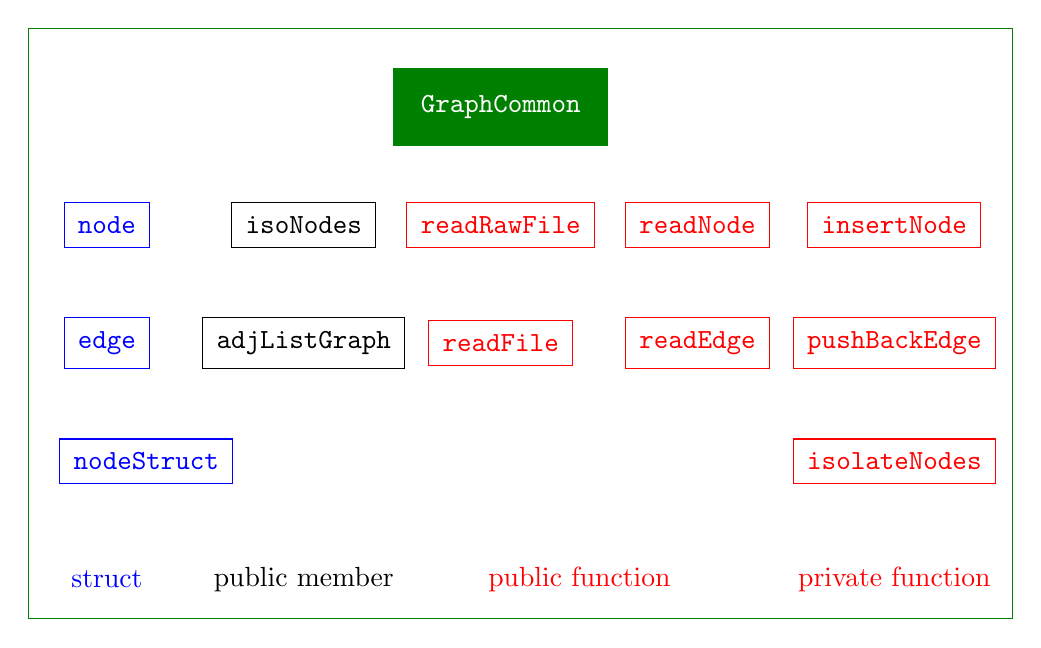
\begin{tikzpicture}
\tikzstyle{class} = [font=\ttfamily\bfseries,color=white,fill=green!50!black,inner sep=10];
\tikzstyle{struct} = [font=\ttfamily\bfseries,color=blue,draw=blue, inner sep = 5];
\tikzstyle{member} = [font=\ttfamily,draw, inner sep=5]
\tikzstyle{function} = [font=\ttfamily\bfseries,color=red,draw=red, inner sep = 5];
\node [class] at (-2,3.5) {GraphCommon};
\node [struct] at (-7,2) {node};
\node [struct] at (-7,0.5) {edge};
\node [struct] at (-6.5,-1) {nodeStruct};
\node [member] at (-4.5,2) {isoNodes};
\node [member] at (-4.5,0.5) {adjListGraph};
\node [function] at (-2,0.5) {readFile};
\node [function] at (-2,2) {readRawFile};
\node [function] at (0.5,2) {readNode};
\node [function] at (0.5,0.5) {readEdge};
\node [function] at (3,2) {insertNode};
\node [function] at (3,0.5) {pushBackEdge};
\node [function] at (3,-1) {isolateNodes};
\draw [green!50!black]  (-8,4.5) rectangle (4.5,-3);
\node [blue] at (-7,-2.5) {struct};
\node at (-4.5,-2.5) {public member};
\node [red] at (-1,-2.5) {public function};
\node [red] at (3,-2.5) {private function};
\end{tikzpicture}
    \caption{\texttt{GraphCommon} 类的成员}
\end{figure}


\subsection{结构体}

该类定义了三个小结构体:
\begin{itemize}
    \item 节点类 \texttt{node}
    \item 有向边类 \texttt{edge}
    \item 节点结构 \texttt{nodeStruct}(用于计算邻接矩阵)
\end{itemize}

前两个都重载了输入输出运算符,以符合目标格式。

\begin{table}[H]
    \centering
    \caption{格式定义}
    \begin{tabular}{cll}{}
        &输入&输出\\
        \hline
        \texttt{node}&$\langle$\texttt{P1}$\rangle$&$\langle$1$\rangle$\\
        \texttt{edge}&$\langle$\texttt{P1 P2 2.0}$\rangle$&$\langle$\texttt{1,2,2.0}$\rangle$\\
        \hline
    \end{tabular}
\end{table}


前缀符号以及分割符可以在后面调整。值得一提的是,优化后子图的虚边定义为如下的格式:
\begin{center}
    \begin{verbatim}
        <起始点,虚点符号,<文件名.终止节点,权重>>
        <1,-1,<O1.2,2.0>>
        \end{verbatim}
\end{center}
在本程序中,\texttt{-1}被定义虚节点符号。

节点结构中定义了三个成员:
\begin{itemize}
    \item \texttt{node Node;} 邻接矩阵边存储
    \item \texttt{map<int, double> adjMatCol;} 邻接矩阵列数值
    \item \texttt{double totalWeight = 0;} 节点发出边总权重
\end{itemize}

并通过三个私有函数同步更新这些数值。

\subsection{公共成员}

该类定义了两个公共成员:
\begin{itemize}
    \item \texttt{set<int> isoNodes} 包含了所有的孤立节点(isolated nodes),也就是完全不连通的部分。
    \item \texttt{map<int, vector<edge>> adjListGraph},邻接表图,仅包含连通部分节点,对于有些连通节点可能为发出空边的集合,即 \texttt{adjListGraph[node] = vector<edge>({});}。
\end{itemize}

\subsection{公共函数}

该类定义了四个公共函数。
\begin{itemize}
    \item \texttt{readNode} 通过输入文本流读取明确定义的节点信息
    \item \texttt{readEdge} 通过文本流读取有向边的信息。
    \item \texttt{readFile} 通过文本流读取文件信息。
    \item \texttt{readRawFile} 通过文本流读取特定格式的文件信息。
\end{itemize}

\subsection{私有函数}

该类定义了三个私有函数。
\begin{itemize}
    \item \texttt{insertNode} 插入节点,包含了对虚节点的检查机制。
    \item \texttt{pushBackEdge} 向邻接表插入边,也包含了对节点是否为虚节点的转换检查机制。
    \item \texttt{isolateNodes} 将 \texttt{readNode} 后的集合去除根据 \texttt{readEdge} 所读取的连接边点,变为孤立节点的集合。
\end{itemize}


\section{图生成器 \texttt{GraphGen}}

图生成器的类 \texttt{GraphGen} 是 \texttt{GraphCommonGen} 的派生类。

本程序的图生成器有几个参数需要设置:

\begin{itemize}
\item
  \textbf{节点类型} \texttt{nodeType}:\texttt{continuous}连续编号的,
  \texttt{discrete}离散的。
\item
  \textbf{边生成类型} \texttt{edgeType}:\texttt{Tree}树(不含环路),
  \texttt{Graph}图(带有环路)。
\item
  \textbf{连通图类型} \texttt{isoType}:\texttt{Single} 单个连通图,
  \texttt{Multi} 多个连通图。
\item
  \textbf{节点编号增长量}
  \texttt{MAX\_INCREASEMENT}:在离散编号模式下,每次生成一个节点都会增长一个数字,这个数字不会超过最大增长量
  。
\item
  \textbf{最大孩子数}
  \texttt{MAX\_CHILD}:每个节点的发出有向边个数不会超过最大孩子数 。
\item
  \textbf{最大连通子图数}
  \texttt{MAX\_ISOGRAPH}:在多个连通图生成模式下,每个图的连通子图数不会超过最大连通子图数。
\item
  \textbf{节点行数占比}
  \texttt{Node\ /\ Lines}:在新文件模式下,仍然会生成随机个数的节点数,但是只输出占比量的节点行数,其余为有向边的行。
\end{itemize}

该程序将会根据上述参数,递增而随机地生成节点编号。然后通过层序遍历生成各个边,如果没有环路的限制,则有可能随机到一个环路节点上去。

随机数采用下面的代码生成:

\begin{lstlisting}
srand((unsigned)time(0)*(++gseed));
return 1.0 * rand() / RAND_MAX;	
\end{lstlisting}

当然,这种方式依然不是特别特别随机,但已经足够。

\section{图分解器 \texttt{GraphDecomp}}

\begin{figure}[H]
    \centering
    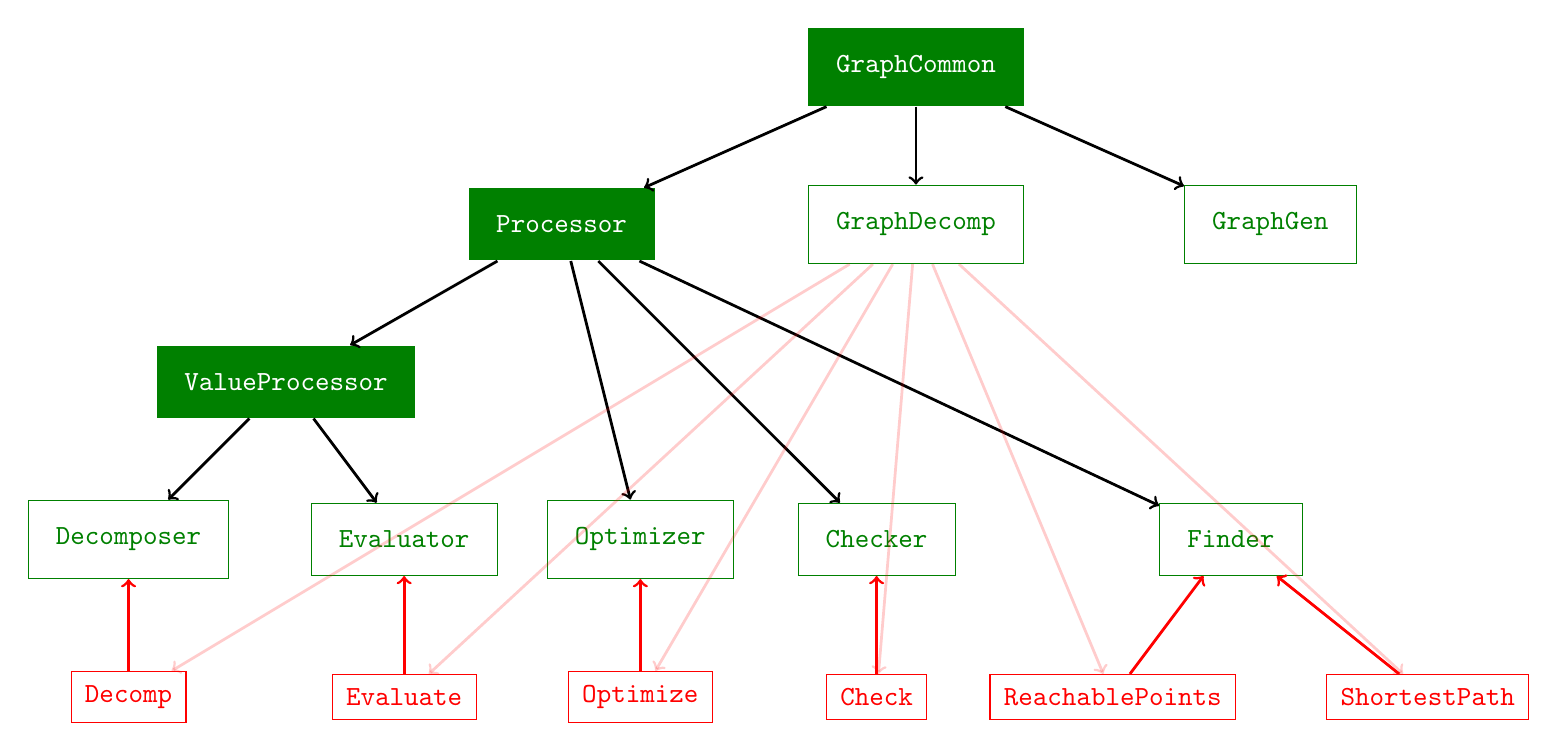
\begin{tikzpicture}
\tikzstyle{class} = [font=\ttfamily\bfseries,color=white,fill=green!50!black,inner sep=10];
\tikzstyle{struct} = [font=\ttfamily\bfseries,color=blue,draw=blue, inner sep = 5];
\tikzstyle{member} = [font=\ttfamily,draw, inner sep=5]
\tikzstyle{function} = [font=\ttfamily\bfseries,color=red,draw=red, inner sep = 5];
\tikzstyle{subclass} = [font=\ttfamily\bfseries,color=green!50!black,draw=green!50!black,inner sep=10];
\tikzstyle{arr} = [line width=1,->];
\tikzstyle{callarr} = [line width=1,->,red];
\tikzstyle{callarrl} = [line width=1,->,red,opacity=0.2];
\node [class] (v1) at (6,4) {GraphCommon};
\node [class] (v2) at (1.5,2) {Processor};
\node [class] (v3) at (-2,0) {ValueProcessor};
\node [subclass] (v4) at (-4,-2) {Decomposer};
\node [subclass] (v5) at (-0.5,-2) {Evaluator};
\node [subclass] (v6) at (2.5,-2) {Optimizer};
\node [subclass] (v7) at (5.5,-2) {Checker};

\node [subclass] (v8) at (10,-2) {Finder};
\draw[arr]  (v1) edge (v2);
\draw [arr] (v2) edge (v3);
\draw [arr] (v3) edge (v4);
\draw [arr] (v3) edge (v5);
\draw [arr] (v2) edge (v6);
\draw [arr] (v2) edge (v7);
\draw [arr] (v2) edge (v8);
\node [subclass] (v15) at (6,2) {GraphDecomp};
\node [function] (v9) at (-4,-4) {Decomp};
\node [function] (v12) at (5.5,-4) {Check};
\node [function] (v11) at (2.5,-4) {Optimize};
\node [function] (v13) at (8.5,-4) {ReachablePoints};
\node [function] (v14) at (12.5,-4) {ShortestPath};
\node [function] (v10) at (-0.5,-4) {Evaluate};
\draw [callarr] (v9) edge (v4);
\draw [callarr] (v10) edge (v5);
\draw [callarr] (v11) edge (v6);
\draw [callarr] (v12) edge (v7);
\draw [callarr] (v13) edge (v8);
\draw [callarr] (v14) edge (v8);
\draw [callarrl] (v15) edge (v9);
\draw [callarrl] (v15) edge (v10);
\draw [callarrl] (v15) edge (v11);
\draw [callarrl] (v15) edge (v12);
\draw [callarrl] (v15) edge (v13);
\draw [callarrl] (v15) edge (v14);
\draw [arr] (v1) edge (v15);
\node [subclass] (v16) at (10.5,2) {GraphGen};
\draw [arr] (v1) edge (v16);
\end{tikzpicture}
    \caption{\texttt{GraphDecomp} 类的成员}
\end{figure}

图分解器类 \texttt{GraphDecomp} 是 \texttt{GraphCommon}
的派生类,为前端提供提供统一接口。

处理器类 \texttt{Processor} 同样是 \texttt{GraphCommon}
的派生类,提供文件处理相关的函数。

值处理器类 \texttt{ValueProcessor} 是 \texttt{Processor}
的派生类,提供邻接矩阵计算相关的函数。

\hypertarget{header-n135}{%
\subsection{\texorpdfstring{分解器
\texttt{Decomposer}}{分解器 Decomposer}}\label{header-n135}}

分解器类 \texttt{Decomposer} 是 \texttt{ValueProcessor} 的派生类,采用
Kerninghan-Lin
算法\cite{kl},将其改进为有向边算法。

对于两节点有向边的损失,可以作为无向边处理,在本程序中定义损失为:
\begin{equation}
    c_{ab} = c_{\overline{ab}}+c_{\overline{ba}}
\end{equation}

对于两个集合$A,B$,各个集合中的对应边$a,b$,将\textbf{外损失}定义为:\begin{equation}
    E_a=\sum_{y \in B}c_{ay}
\end{equation}

\textbf{内损失}定义为:
\begin{equation}
    I_a=\sum_{x \in A}c_{ax}
\end{equation}

\textbf{内外差}定义为:
\begin{equation}
    D_z = E_z - I_z, \forall z \in S
\end{equation}

\textbf{损失缩减量}定义为:
\begin{equation}
    g_{ab} = D_a + D_b - 2c_{ab}
\end{equation}

可以设置算法的猛烈程度
\texttt{DecompSol},来影响分解时间和分解效果,对于大规模运算集会有显著的影响:

\begin{itemize}
\item
  \texttt{rough} 按照顺序分割,最快(\texttt{order})。
\item
  \texttt{bfs} 采用广度优先搜索算法,快一些(\texttt{bfs})。
\item
  \texttt{onepass} 每次只进行一次优化,居中(\texttt{medium})。
\item
  \texttt{ll} 取用局部最优($D$ 优先算法),慢一些(\texttt{harder})。
\item
  \texttt{kl} 标准算法,强力优化($g$ 优先算法),最慢(\texttt{hardest})。
\end{itemize}

Kerninghan-Lin 算法的主要过程:对于两个分割集合$A$,$B$,循环以下过程:

\begin{algorithm}[H]
    \KwIn{需要被优化的分割集合 $A,B$}
    \KwOut{被优化后的分割集合 $A,B$}
    \BlankLine
    \caption{修改后的 Kerninghan-Lin 算法} \label{Alg-KL}
    \Repeat{$G\leq 0$}{
        对于分割集 $A,B$ 中的每个元素计算 $D$\;
        $p\leftarrow 1$\;
        $A_p\leftarrow A, B_p\leftarrow B$\;
        \Repeat{$p=|A|$}{
            \nlset{ll} 选择 $a_i\in A_p, b_j\in B_p$ 使得 $g_p=D_{a_i}+D_{b_j}-2c_{a_ib_j}$最大\;
            $a_p^\prime\leftarrow a_i$\;
            $b_p^\prime\leftarrow b_j$\;
            \nlset{MOD} $A_{p+1}\leftarrow A_p - \{a_i\} + \{b_j\}$\;
            \nlset{MOD} $B_{p+1}\leftarrow B_p + \{a_i\} - \{b_j\}$\;
            $p\leftarrow p+1$\;
            对于分割集 $A_p,B_p$ 中的每个元素计算 $D$\;
        }
        选择$k$使得$G=\sum_{i=1}^k g_i$最大\;
        \nlset{onepass} \uIf{$G\leq 0$}{
            \textbf{break}\;
        }
        $A\leftarrow A - \{a_1^\prime,a_2^\prime,\cdots a_k^\prime\} + \{b_1^\prime,b_2^\prime,\cdots,b_k^\prime\}$\;
        $B\leftarrow B + \{a_1^\prime,a_2^\prime,\cdots a_k^\prime\} - \{b_1^\prime,b_2^\prime,\cdots,b_k^\prime\}$\;
    }
\end{algorithm}

在 Kerninghan-Lin 的原算法中,是需要在 \textbf{MOD} 中直接去除两个元素,但是实验证明这么做的效果对有向边没有这种好,因为计算 $G$ 的意义就是为了看交换到哪一步就是最好的优化,而在我们需要保持原集合大小不变的情况下,不应当在算法中间尝试减少集合的大小。

\begin{itemize}
\item
  \texttt{kl} 模式就是采用上述算法。
\item
  \texttt{ll}
  模式对步骤 \textbf{ll} 进行了改进,仅仅通过选择两个集合中最大的 $D$ 对应的元素进行交换。
\item
  \texttt{onepass}
  对步骤 \textbf{onepass} 进行放宽,只进行一次优化,就退出。对于步骤5只重复原次数的四分之一。
\item
  \texttt{bfs}
  直接采用广度优先搜索,每次选择最大连接权重的节点遍历其子节点,直至每个集合达到集合个数上限。
\item
  \texttt{rough} 模式就是对集合进行顺序二分,直至集合大小符合要求。
\end{itemize}

节点分配完毕后,将会将节点及其\textbf{所有}发出边存储在对应文件中。

\hypertarget{header-n185}{%
\subsubsection{\texorpdfstring{评估器
\texttt{Evaluater}}{评估器 Evaluater}}\label{header-n185}}

对于外部分解文件的评估,该评估器定义节点的存储位置优先级如下:

\begin{enumerate}
\def\labelenumi{\arabic{enumi}.}
\item
  对于以节点形式存储的节点,存在对应的文件中
\item
  对于第一次以有向边起点存储的节点,存在对应的文件中
\item
  连通节点中的叶子节点将会存储在最后一次出现的文件中
\end{enumerate}

独立的评估器类为 \texttt{Evaluater},当然 \texttt{Decomposer}
内会在完成分割后进行评估。但主要的评估函数 \texttt{Evaluate()}
都来自于父类 \texttt{ValueProcessor}。

首先需要计算每一对元素的邻接权重矩阵,需要进行 $n^2$ 次计算。

如果将 $n$ 个元素几乎平均地分配到元素个数为$|P|$个集合中,共有 $\frac{n}{|P|}$ 个集合,则需要进行对每两个集合间的每两个元素计算,需要 $C_{\frac{n}{|P|}}^2|P|^2=O(n^2)$ 次计算,算出损失值。

最后计算总权重,计算损失矩阵上对角线部分(包含对角线)的和。

该运算的成本较高,设置了 \texttt{CALC\ afer\ DECOMP}
选项以选择跳过计算权重部分。

\hypertarget{header-n199}{%
\subsection{\texorpdfstring{优化器
\texttt{Optimizer}}{优化器 Optimizer}}\label{header-n199}}

优化器 \texttt{Optimizer} 是 \texttt{Processor} 的子类。

由本程序产生的分解子图,都会将节点存储位置以节点形式存储在对应文件中。优化器仅仅优化末尾节点,使其指向虚节点,并存储对应的文件位置。

分解器保证了所有的节点及其发出边都在同一个文件中,所以起始节点不会为虚节点。而如果起始节点为虚节点,将会对后面的寻找可达节点和最短路径造成极大的障碍,因为就难以预料起始节点在哪些文件中,最终很有可能沦为变相合并子图的过程,将会不符合题意。所以该程序限制只有终止节点为虚节点。

\hypertarget{header-n203}{%
\subsection{\texorpdfstring{检查器
\texttt{Checker}}{检查器 Checker}}\label{header-n203}}

检查器 \texttt{Checker} 是 \texttt{Processor}
的子类,用以检查主图与分解图、分解图与优化图之间是否存储一致。重载了集合比较函数,定义了映射比较函数,用于比较两者的鼓励节点存储与邻接表图存储是否都是一致的。

\hypertarget{header-n206}{%
\subsection{\texorpdfstring{访达器
\texttt{Finder}}{访达器 Finder}}\label{header-n206}}

访达器 \texttt{Finder} 是 \texttt{Processor}
的子类,用于寻找可达节点与最短路径。

\hypertarget{header-n208}{%
\subsubsection{\texorpdfstring{可达节点
\texttt{ReachablePoints}}{可达节点 ReachablePoints}}\label{header-n208}}

本程序所生成的优化后子图文件,节点存储位置将会存储所有发出边,虚节点只适用于有向边结束节点。因此,在这种限制规则下,可以将文件视作\textbf{广义节点},当访问该点时出现虚边指出该文件,则输入文件访问队列,在该文件访问完毕后,访问队列中的下一个文件以及相应的节点。这样就可以在子图访问的前提下,获取所有的可达节点。

当然使用该算法会导致读取不同格式的子图文件做寻找算法时出现找不全的情形(比如起始节点为虚节点的情形)。

\hypertarget{header-n211}{%
\subsubsection{\texorpdfstring{最短路径
\texttt{ShortestPath}}{最短路径 ShortestPath}}\label{header-n211}}

采用 SPFA(Shortest Path Faster Algorithm) 算法。仍然在只有终止节点为虚节点的限制下,仿照上述可达节点的做法依次访问从起始节点开始的所有可达节点,每访问一个节点,都会考虑从上一个节点通过该有向边能否比原来的权重更少,如果是,则更新该节点的权重值,并存储路径到 \texttt{prev} 中,并放入访问队列中。

SPFA 在形式上和 BFS 非常类似,不同的是 BFS 中一个点出了队列就不可能重新进入队列,但是 SPFA 中一个点可能在出队列之后再次被放入队列,也就是一个点改进过其它的点之后,过了一段时间可能本身被改进,于是再次用来改进其它的点,这样反复迭代下去。这种算法相比于
dijkstra 更适合于多子图上最短路径的寻找,没有使用排除访问的方法。

\section{性能评估}

通过图生成器生成了 9 个图文件,之后通过图分解器分解为原图规模的 5 \%,计时并查看结果。

\begin{table}[H]
    \centering
    \caption{分解优化检查性能结果}
    \begin{tabular}{c|rrrrr|rrrrr}{}
    &\multicolumn{5}{c}{分解优化检查时间(s)} & \multicolumn{5}{c}{分解优化检查割边比例} \\
    规模 & \texttt{hardest} & \texttt{harder} & \texttt{medium} & \texttt{bfs} & \texttt{order} & \texttt{hardest} & \texttt{harder} & \texttt{medium} & \texttt{bfs} & \texttt{order} \\
    \hline
    100 & 0.5 &0.5 &0.5	&0.5	&0.5 & 16.7\% & 41.7\% & 41.6\% & 50.0\% & 75.0\% \\
    200 & 1	&1	&1	&1	&1 & 39.2\% & 38.4\% & 46.6\% & 67.7\% & 71.9\% \\
    300 & 1 &1	&1	&1	&1 & 44.9\% & 47.0\% & 52.6\% & 65.0\% & 77.4\% \\
    500 &1	&1	&1	&1	&1  & 55.1\% & 56.9\% & 65.2\% & 66.6\% & 85.4\% \\
    1000 &3	&3	&2	&1	&1 & 51.5\% & 51.7\% & 62.7\% & 65.5\% & 90.3\% \\
    2000 &12	&9	&3	&1	&1 & 35.2\% & 36.7\% & 44.6\% & 60.4\% & 73.7\% \\
    3000 &33	&24	&6.5	&1	&1 & 33.9\% & 32.9\% & 43.3\% & 59.8\% & 75.5\% \\
    5000 &133	&90	&21	&1.5	&1 & 39.5\% & 38.8\% & 46.7\% & 54.2\% & 75.4\% \\
    10000 &1020	&736	&180	&2.4	&2 & 9.2\% & 8.7\% & 27.0\% & 49.2\% & 74.5\% \\
    \hline
    \end{tabular}
\end{table}

以 \texttt{order} 模式为基准,考察其余模式下的时间与效果优化程度。定义性价比为:
\begin{equation}
    \text{Value} = \frac{\rm Effect}{\rm Time} = \frac{\frac{1}{\rm Cut~Edge~Proportion}}{\rm Time~Magnification}
\end{equation}

\begin{figure}[H]
    \centering
    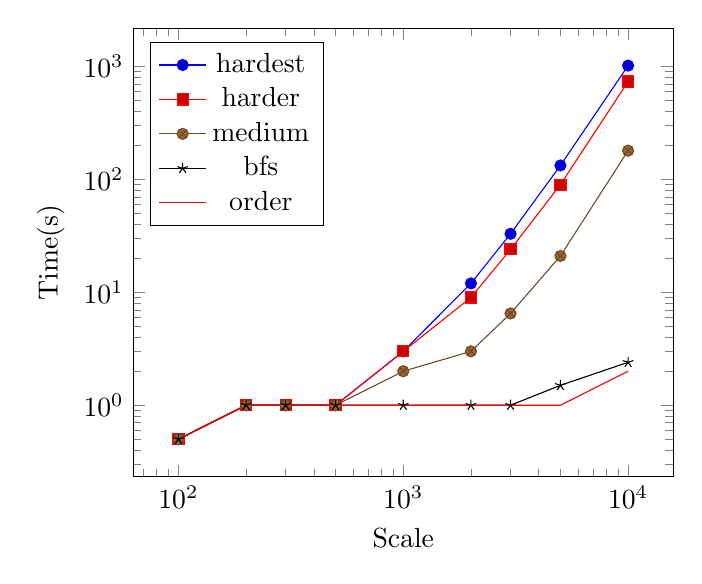
\begin{tikzpicture}
    \pgfplotstableread [row sep=crcr]
    {scale hardest harder medium bfs order\\100 0.5 0.5 0.5 0.5 0.5\\200 1 1 1 1 1\\300 1 1 1 1 1\\500 1 1 1 1 1\\1000 3 3 2 1 1\\2000 12 9 3 1 1\\3000 33 24 6.5 1 1\\5000 133 90 21 1.5 1\\10000 1020 736 180 2.4 2\\\\}
    {\value}
    \begin{loglogaxis}[legend pos=north west,
    ylabel={Time(s)},
    xlabel={Scale},]
     \addplot+ [] table[y=hardest] {\value};
     \addplot+ [] table[y=harder] {\value};
    \addplot+ [] table[y=medium] {\value};
    \addplot+ [] table[y=bfs] {\value};
    \addplot[red] table[y=order] {\value};
    \legend{hardest,harder,medium,bfs,order};
    \end{loglogaxis}
\end{tikzpicture}
    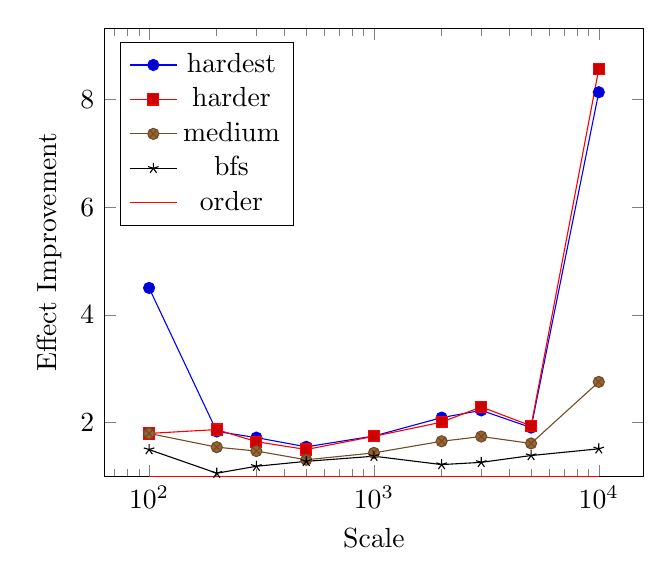
\begin{tikzpicture}
\pgfplotstableread [row sep=crcr]
{scale hardest harder medium bfs order\\100 4.5 1.8 1.8 1.5 1\\200 1.836477987 1.871794872 1.544973545 1.061818182 1\\300 1.722222222 1.64665127 1.473140496 1.190317195 1\\500 1.551309271 1.501369863 1.311004785 1.281871345 1\\1000 1.751718869 1.746382331 1.438745098 1.376970425 1\\2000 2.0928277 2.009021842 1.654457769 1.221831833 1\\3000 2.227881723 2.291983122 1.742461736 1.262780348 1\\5000 1.908465831 1.94093311 1.61437736 1.389680633 1\\10000 8.131952564 8.563129127 2.756167342 1.514154272 1\\\\}
{\value}
\begin{semilogxaxis}[legend pos=north west,
ylabel={Effect Improvement},
xlabel={Scale},
ymin=1]
 \addplot+ [] table[y=hardest] {\value};
 \addplot+ [] table[y=harder] {\value};
\addplot+ [] table[y=medium] {\value};
\addplot+ [] table[y=bfs] {\value};
\addplot[red] table[y=order] {\value};
\legend{hardest,harder,medium,bfs,order};
\end{semilogxaxis}
\end{tikzpicture}
    \caption{不同规模下的时间和效果提升图}
\end{figure}

\begin{figure}[H]
    \centering
    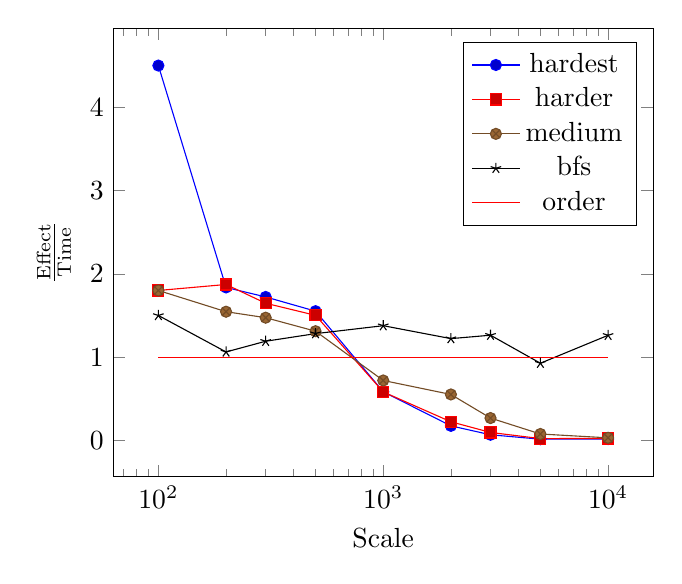
\begin{tikzpicture}
\pgfplotstableread [row sep=crcr]
{scale hardest harder medium bfs order\\100 4.5 1.8 1.8 1.5 1\\200 1.836477987 1.871794872 1.544973545 1.061818182 1\\300 1.722222222 1.64665127 1.473140496 1.190317195 1\\500 1.551309271 1.501369863 1.311004785 1.281871345 1\\1000 0.58390629 0.582127444 0.719372549 1.376970425 1\\2000 0.174402308 0.223224649 0.551485923 1.221831833 1\\3000 0.067511567 0.095499297 0.268071036 1.262780348 1\\5000 0.014349367 0.021565923 0.076875112 0.926453755 1\\10000 0.015945005 0.023269373 0.030624082 1.261795227 1\\\\}
{\value}
\begin{semilogxaxis}[legend pos=north east,
ylabel={$\frac{\rm Effect}{\rm Time}$},
xlabel={Scale}]
 \addplot+ [] table[y=hardest] {\value};
 \addplot+ [] table[y=harder] {\value};
\addplot+ [] table[y=medium] {\value};
\addplot+ [] table[y=bfs] {\value};
\addplot[red] table[y=order] {\value};
\legend{hardest,harder,medium,bfs,order};
\end{semilogxaxis}
\end{tikzpicture}
    \caption{不同规模下的性价比图}
\end{figure}

在评测时,20s 左右都是可以接受的,所以:
\begin{itemize}
    \item 对于 $0\leq n\leq 1000$ 的图,都可以使用 \texttt{hardest} 模式,以期获得更好的分解效果。
    \item 对于 $1000 < n\leq 3000$ 的图,都可以使用 \texttt{harder} 模式,时间上不仅可以缩减为 \texttt{hardest} 的 $\frac{2}{3}$,效果上甚至可能会比 \texttt{hardest} 的要略好,因为都是局部最优算法,并不一定是全局最优。
    \item 对于 $3000 < n \leq 7000$ 的图,都可以使用 \texttt{medium} 模式,进一步缩减时间,并保证比 \texttt{harder} 更高的性价比。
    \item 对于 $n > 7000$ 的图,使用 \texttt{bfs} 模式节约时间,Kerninghan-Lin 算法所需要的时间过长,尽管效果提升可能比较明显。但是 \texttt{bfs} 模式 可以保证平稳的 50 \% 割边比例,也即保证基线的 $\frac{1}{3}$ 优化率。
    \item 如果分割限制比例向下调整,则算法就需要降档,以满足时间限制。当然,从时间复杂度的分析来看,分割成过细的子图会导致评估割边权重部分耗费过多的时间,可以考虑关闭 \texttt{CLAC after DECOMP} 选项以期大幅减少时间耗费量与内存占用率。
\end{itemize}

\bibliography{ref}

\end{CJK}
\end{document}